\section{\RU{Строки}\EN{Strings}}
\label{sec:digging_strings}

\EN{\section{Text strings}

\subsection{\CCpp}

\label{C_strings}
The normal C strings are zero-terminated (\ac{ASCIIZ}-strings).

The reason why the C string format is as it is (zero-terminated) is apparently historical.
In [Dennis M. Ritchie, \IT{The Evolution of the Unix Time-sharing System}, (1979)]
we read:

\begin{framed}
\begin{quotation}
A minor difference was that the unit of I/O was the word, not the byte, because the PDP-7 was a word-addressed
machine. In practice this meant merely that all programs dealing with character streams ignored null
characters, because null was used to pad a file to an even number of characters.
\end{quotation}
\end{framed}

\myindex{Hiew}

In Hiew or FAR Manager these strings looks like this:

\begin{lstlisting}
int main()
{
	printf ("Hello, world!\n");
};
\end{lstlisting}

\begin{figure}[H]
\centering
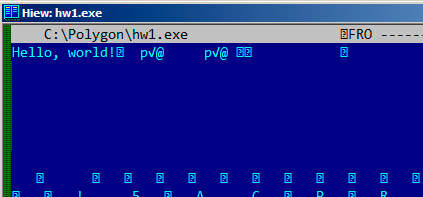
\includegraphics[scale=\NormalScale]{digging_into_code/strings/C-string.png}
\caption{Hiew}
\end{figure}

% FIXME видно \n в конце, потом пробел

\subsection{Borland Delphi}
\myindex{Pascal}
\myindex{Borland Delphi}

The string in Pascal and Borland Delphi is preceded by an 8-bit or 32-bit string length.

For example:

\begin{lstlisting}[caption=Delphi]
CODE:00518AC8                 dd 19h
CODE:00518ACC aLoading___Plea db 'Loading... , please wait.',0

...

CODE:00518AFC                 dd 10h
CODE:00518B00 aPreparingRun__ db 'Preparing run...',0
\end{lstlisting}

\subsection{Unicode}

\myindex{Unicode}

Often, what is called Unicode is a methods for encoding strings where each character occupies 2 bytes or 16 bits.
This is a common terminological mistake.
Unicode is a standard for assigning a number to each character in the many writing systems of the 
world, but does not describe the encoding method.

\myindex{UTF-8}
\myindex{UTF-16LE}
The most popular encoding methods are: UTF-8 (is widespread in Internet and *NIX systems) and UTF-16LE (is used in Windows).

\subsubsection{UTF-8}

\myindex{UTF-8}
UTF-8 is one of the most successful methods for
encoding characters.
All Latin symbols are encoded just like in ASCII,
and the symbols beyond the ASCII table are encoded using several bytes.
0 is encoded as
before, so all standard C string functions work with UTF-8 strings just like any other string.

Let's see how the symbols in various languages are encoded in UTF-8 and how it looks like in FAR, using the 437 codepage
\footnote{The example and translations was taken from here: 
\url{http://go.yurichev.com/17304}}:

\begin{figure}[H]
\centering
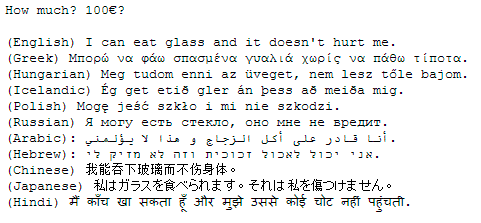
\includegraphics[scale=\NormalScale]{digging_into_code/strings/multilang_sampler.png}
\end{figure}

% FIXME: cut it
\begin{figure}[H]
\centering
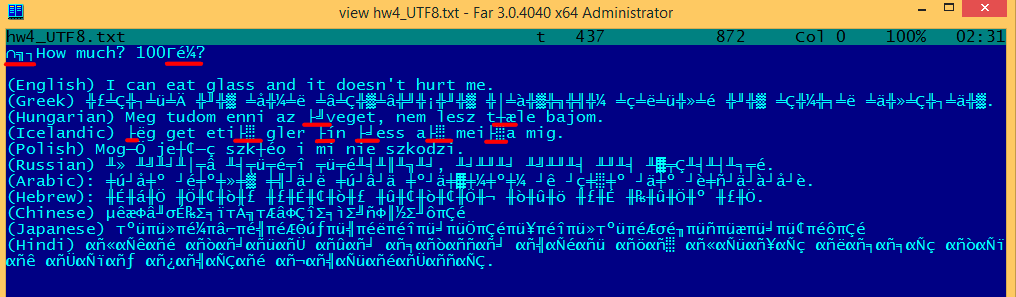
\includegraphics[scale=\FigScale]{digging_into_code/strings/multilang_sampler_UTF8.png}
\caption{FAR: UTF-8}
\end{figure}

As you can see, the English language string looks the same as it is in ASCII.

The Hungarian language uses some Latin symbols plus symbols with diacritic marks.

These symbols are encoded using several bytes, these are underscored with red.
It's the same story with the Icelandic and Polish languages.

There is also the \q{Euro} currency symbol at the start, which is encoded with 3 bytes.

The rest of the writing systems here have no connection with Latin.

At least in Russian, Arabic, Hebrew and Hindi we can see some recurring bytes, and that is not surprise:
all symbols from a writing system are usually located in the same Unicode table, so their code begins with
the same numbers.

At the beginning, before the \q{How much?} string we see 3 bytes, which are in fact the \ac{BOM}.
The \ac{BOM} defines the encoding system to be
used.

\subsubsection{UTF-16LE}

\myindex{UTF-16LE}
\myindex{Windows!Win32}
Many win32 functions in Windows have the suffixes \TT{-A} and \TT{-W}.
The first type of functions works
with normal strings, the other with UTF-16LE strings (\IT{wide}).

In the second case, each symbol is usually stored in a 16-bit value of type \IT{short}.

The Latin symbols in UTF-16 strings look in Hiew or FAR like they are interleaved with zero byte:

\begin{lstlisting}
int wmain()
{
	wprintf (L"Hello, world!\n");
};
\end{lstlisting}

\begin{figure}[H]
\centering
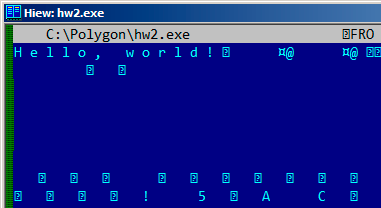
\includegraphics[scale=\NormalScale]{digging_into_code/strings/UTF16-string.png}
\caption{Hiew}
\end{figure}

We can see this often in \gls{Windows NT} system files:

\begin{figure}[H]
\centering
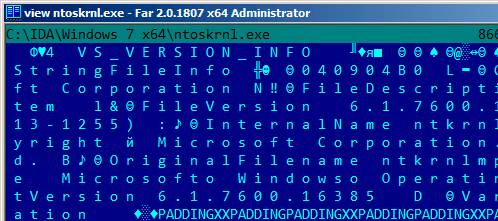
\includegraphics[scale=\NormalScale]{digging_into_code/strings/ntoskrnl_UTF16.png}
\caption{Hiew}
\end{figure}

\myindex{IDA}
Strings with characters that occupy exactly 2 bytes are called \q{Unicode} in \IDA:

\begin{lstlisting}
.data:0040E000 aHelloWorld:
.data:0040E000                 unicode 0, <Hello, world!>
.data:0040E000                 dw 0Ah, 0
\end{lstlisting}

Here is how the Russian language string is encoded in UTF-16LE:

\begin{figure}[H]
\centering
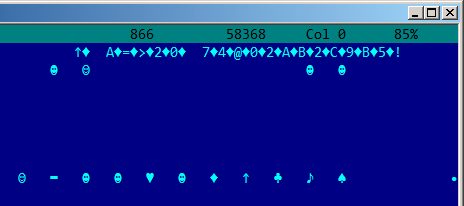
\includegraphics[scale=\NormalScale]{digging_into_code/strings/russian_UTF16.png}
\caption{Hiew: UTF-16LE}
\end{figure}

What we can easily spot is that the symbols are interleaved by the diamond character (which has the ASCII code of 4).
Indeed, the Cyrillic symbols are located in the fourth Unicode plane
\footnote{\href{http://go.yurichev.com/17003}{wikipedia}}.
Hence, all Cyrillic symbols in UTF-16LE are located in the \TT{0x400-0x4FF} range.

Let's go back to the example with the string written in multiple languages.
Here is how it looks like in UTF-16LE.

% FIXME: cut it
\begin{figure}[H]
\centering
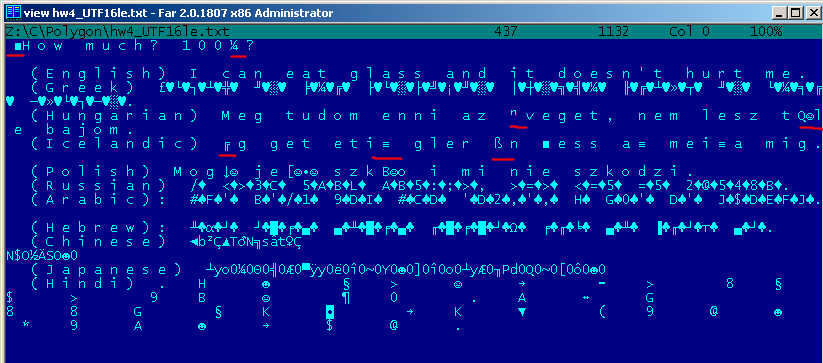
\includegraphics[scale=\FigScale]{digging_into_code/strings/multilang_sampler_UTF16.png}
\caption{FAR: UTF-16LE}
\end{figure}

Here we can also see the \ac{BOM} in the beginning.
All Latin characters are interleaved with a zero byte.

Some characters with diacritic marks (Hungarian and Icelandic languages) are also underscored in red.

% TODO: strings *NIX utility. procmonitor also shows strings...

% subsection:
\subsection{Base64}
\myindex{Base64}

The base64 encoding is highly popular for the cases when you need to transfer binary data as a text string.

In essence, this algorithm encodes 3 binary bytes into 4 printable characters:
all 26 Latin letters (both lower and upper case), digits, plus sign (\q{+}) and slash sign (\q{/}),
64 characters in total.

One distinctive feature of base64 strings is that they often (but not always) ends with 1 or 2 \gls{padding}
equality symbol(s) (\q{=}), for example:

\begin{lstlisting}
AVjbbVSVfcUMu1xvjaMgjNtueRwBbxnyJw8dpGnLW8ZW8aKG3v4Y0icuQT+qEJAp9lAOuWs=
\end{lstlisting}

\begin{lstlisting}
WVjbbVSVfcUMu1xvjaMgjNtueRwBbxnyJw8dpGnLW8ZW8aKG3v4Y0icuQT+qEJAp9lAOuQ==
\end{lstlisting}

The equality sign (\q{=}) is never encounter in the middle of base64-encoded strings.

Now example of manual encoding.
Let's encode 0x00, 0x11, 0x22, 0x33 hexadecimal bytes into base64 string:

\lstinputlisting{digging_into_code/strings/base64_ex.sh}

Let's put all 4 bytes in binary form, then regroup them into 6-bit groups:

\begin{lstlisting}
|  00  ||  11  ||  22  ||  33  ||      ||      |
00000000000100010010001000110011????????????????
| A  || B  || E  || i  || M  || w  || =  || =  |
\end{lstlisting}

Three first bytes (0x00, 0x11, 0x22) can be encoded into 4 base64 characters (``ABEi''),
but the last one (0x33) --- cannot be,
so it's encoded using two characters (``Mw'') and \gls{padding} symbol (``='')
is added twice to pad the last group to 4 characters.
Hence, length of all correct base64 strings are always divisible by 4.

\myindex{XML}
Base64 is often used when binary data needs to be stored in XML.

Some people tries to use base64 to obfuscate strings:
\url{http://blog.sec-consult.com/2016/01/deliberately-hidden-backdoor-account-in.html}
\footnote{\url{http://archive.is/nDCas}}.

\myindex{base64scanner}
There are utilities for scanning an arbitrary binary files for base64 strings.
One such utilitiy is base64scanner\footnote{\url{https://github.com/dennis714/base64scanner}}.

\myindex{UseNet}
\myindex{FidoNet}
\myindex{Uuencoding}
Another encoding system which was much more popular in UseNet and FidoNet is Uuencoding.
It offers mostly the same features, but is different from base64 in the sense that file name
is also stored in header.


}
\RU{\sectionold{Текстовые строки}

\subsectionold{\CCpp}

\label{C_strings}
Обычные строки в Си заканчиваются нулем (\ac{ASCIIZ}-строки).

Причина, почему формат строки в Си именно такой (оканчивающийся нулем) вероятно историческая.
В [Dennis M. Ritchie, \IT{The Evolution of the Unix Time-sharing System}, (1979)]
мы можем прочитать:

\begin{framed}
\begin{quotation}
A minor difference was that the unit of I/O was the word, not the byte, because the PDP-7 was a word-addressed
machine. In practice this meant merely that all programs dealing with character streams ignored null
characters, because null was used to pad a file to an even number of characters.
\end{quotation}
\end{framed}

\myindex{Hiew}
Строки выглядят в Hiew или FAR Manager точно так же:

\begin{lstlisting}
int main()
{
	printf ("Hello, world!\n");
};
\end{lstlisting}

\begin{figure}[H]
\centering
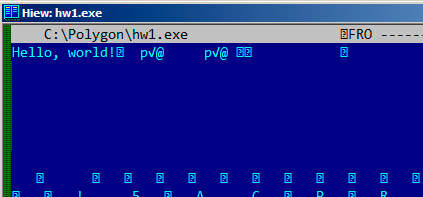
\includegraphics[scale=\NormalScale]{digging_into_code/strings/C-string.png}
\caption{Hiew}
\end{figure}

% FIXME видно \n в конце, потом пробел

\subsectionold{Borland Delphi}
\myindex{Pascal}
\myindex{Borland Delphi}
Когда кодируются строки в Pascal и Delphi, сама строка предваряется 8-битным или 32-битным значением, в котором закодирована длина строки.

Например:

\begin{lstlisting}[caption=Delphi]
CODE:00518AC8                 dd 19h
CODE:00518ACC aLoading___Plea db 'Loading... , please wait.',0

...

CODE:00518AFC                 dd 10h
CODE:00518B00 aPreparingRun__ db 'Preparing run...',0
\end{lstlisting}

\subsectionold{Unicode}

\myindex{Unicode}
Нередко уникодом называют все способы передачи символов, когда символ занимает 2 байта или 16 бит.
Это распространенная терминологическая ошибка.
Уникод --- это стандарт, присваивающий номер каждому символу многих письменностей мира, но не описывающий
способ кодирования.

\myindex{UTF-8}
\myindex{UTF-16LE}
Наиболее популярные способы кодирования: 
UTF-8 (наиболее часто используется в Интернете и *NIX-системах) и UTF-16LE (используется в Windows).

\subsubsectionold{UTF-8}

\myindex{UTF-8}
UTF-8 это один из очень удачных способов кодирования символов.
Все символы латиницы кодируются так же, как и в ASCII-кодировке, а символы, выходящие за пределы
ASCII-7-таблицы, кодируются несколькими байтами.
0 кодируется, как и прежде, нулевыми байтом, так что все стандартные
функции Си продолжают работать с UTF-8-строками так же как и с обычными строками.

Посмотрим, как символы из разных языков кодируются в UTF-8 и как это выглядит в FAR, в кодировке 437

\footnote{Пример и переводы на разные языки были взяты здесь: 
\url{http://go.yurichev.com/17304}}:

\begin{figure}[H]
\centering
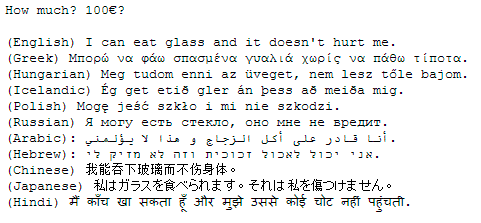
\includegraphics[scale=\NormalScale]{digging_into_code/strings/multilang_sampler.png}
\end{figure}

% FIXME: cut it
\begin{figure}[H]
\centering
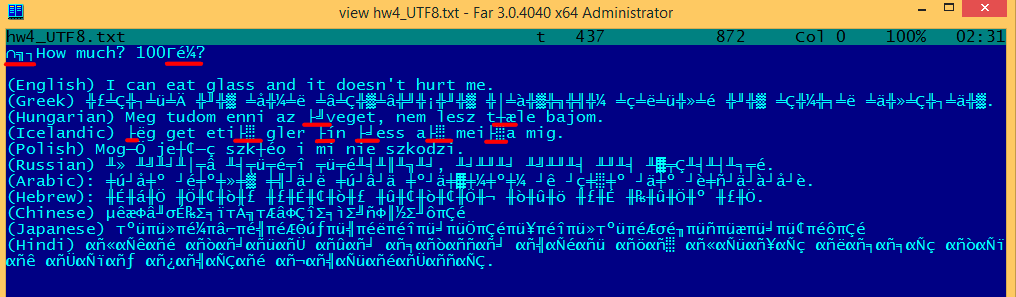
\includegraphics[scale=\FigScale]{digging_into_code/strings/multilang_sampler_UTF8.png}
\caption{FAR: UTF-8}
\end{figure}

Видно, что строка на английском языке выглядит точно так же, как и в ASCII-кодировке.
В венгерском языке используются латиница плюс латинские буквы с диакритическими знаками.
Здесь видно, что эти буквы кодируются несколькими байтами, они подчеркнуты красным.
То же самое с исландским и польским языками.
В самом начале имеется также символ валюты \q{Евро}, который кодируется тремя байтами.
Остальные системы письма здесь никак не связаны с латиницей.
По крайней мере о русском, арабском, иврите и хинди мы можем сказать, что здесь видны повторяющиеся
байты, что не удивительно, ведь, обычно буквы из одной и той же системы письменности расположены в одной
или нескольких таблицах уникода, поэтому часто их коды начинаются с одних и тех же цифр.

В самом начале, перед строкой \q{How much?}, видны три байта, которые на самом деле \ac{BOM}.
\ac{BOM} показывает, какой способ кодирования будет сейчас использоваться.

\subsubsectionold{UTF-16LE}

\myindex{UTF-16LE}
\myindex{Windows!Win32}
Многие функции win32 в Windows имееют суффикс \TT{-A} и \TT{-W}.
Первые функции работают с обычными строками, вторые с UTF-16LE-строками (\IT{wide}).
Во втором случае, каждый символ обычно хранится в 16-битной переменной типа \IT{short}.

Cтроки с латинскими буквами выглядят в Hiew или FAR как перемежающиеся с нулевыми байтами:

\begin{lstlisting}
int wmain()
{
	wprintf (L"Hello, world!\n");
};
\end{lstlisting}

\begin{figure}[H]
\centering
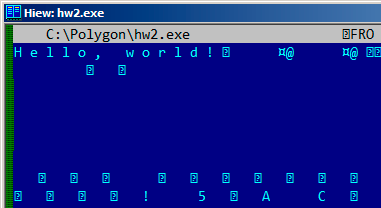
\includegraphics[scale=\NormalScale]{digging_into_code/strings/UTF16-string.png}
\caption{Hiew}
\end{figure}

Подобное можно часто увидеть в системных файлах \gls{Windows NT}:

\begin{figure}[H]
\centering
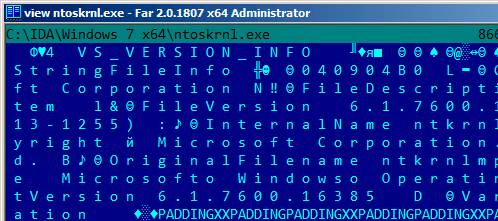
\includegraphics[scale=\NormalScale]{digging_into_code/strings/ntoskrnl_UTF16.png}
\caption{Hiew}
\end{figure}

\myindex{IDA}
В \IDA, уникодом называется именно строки с символами, занимающими 2 байта:

\begin{lstlisting}
.data:0040E000 aHelloWorld:
.data:0040E000                 unicode 0, <Hello, world!>
.data:0040E000                 dw 0Ah, 0
\end{lstlisting}

Вот как может выглядеть строка на русском языке (\q{И снова здравствуйте!}) закодированная в UTF-16LE:

\begin{figure}[H]
\centering
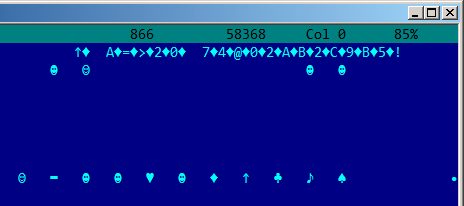
\includegraphics[scale=\NormalScale]{digging_into_code/strings/russian_UTF16.png}
\caption{Hiew: UTF-16LE}
\end{figure}

То что бросается в глаза\EMDASH{}это то что символы перемежаются ромбиками (который имеет код 4).
Действительно, в уникоде кирилличные символы находятся в четвертом блоке
\footnote{\href{http://go.yurichev.com/17003}{wikipedia}}.
Таким образом, все кирилличные символы в UTF-16LE находятся в диапазоне \TT{0x400-0x4FF}.

Вернемся к примеру, где одна и та же строка написана разными языками.
Здесь посмотрим в кодировке UTF-16LE.

% FIXME: cut it
\begin{figure}[H]
\centering
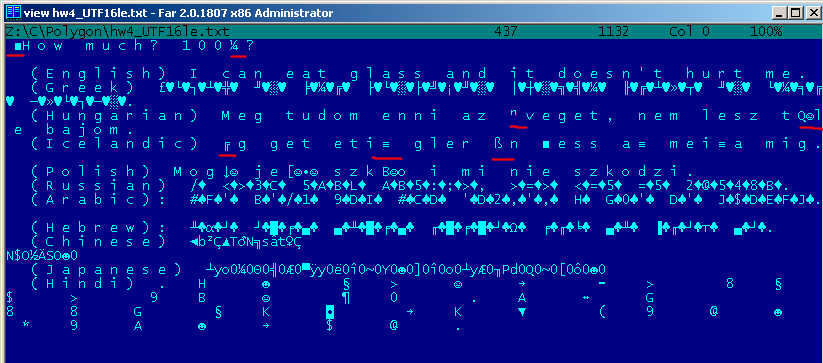
\includegraphics[scale=\FigScale]{digging_into_code/strings/multilang_sampler_UTF16.png}
\caption{FAR: UTF-16LE}
\end{figure}

Здесь мы также видим \ac{BOM} в самом начале.
Все латинские буквы перемежаются с нулевыми байтом.
Некоторые буквы с диакритическими знаками (венгерский и исландский языки) также подчеркнуты красным.

% TODO: strings *NIX utility. procmonitor also shows strings...

% subsection:
\subsection{Base64}
\myindex{Base64}

Кодировка base64 очень популярна в тех случаях, когда нужно передать двоичные данные как текстовую строку.

По сути, этот алгоритм кодирует 3 двоичных байта в 4 печатаемых символа:
все 26 букв латинского алфавита (в обоих регистрах), цифры, знак плюса (\q{+}) и слэша (\q{/}),
в итоге это получается 64 символа.

Одна отличительная особенность строк в формате base64, это то что они часто (хотя и не всегда) заканчиваются
одним или двумя символами знака равенства (\q{=}) для выравнивания (\gls{padding}), например:

\begin{lstlisting}
AVjbbVSVfcUMu1xvjaMgjNtueRwBbxnyJw8dpGnLW8ZW8aKG3v4Y0icuQT+qEJAp9lAOuWs=
\end{lstlisting}

\begin{lstlisting}
WVjbbVSVfcUMu1xvjaMgjNtueRwBbxnyJw8dpGnLW8ZW8aKG3v4Y0icuQT+qEJAp9lAOuQ==
\end{lstlisting}

Так что знак равенства (\q{=}) никогда не встречается в середине строк закодированных в base64.

Теперь пример кодирования вручную.
Попробуем закодировать шестнадцатеричные байты 0x00, 0x11, 0x22, 0x33 в строку в формате base64:

\lstinputlisting{digging_into_code/strings/base64_ex.sh}

Запишем все 4 байта в двоичной форме, затем перегруппируем их в 6-битные группы:

\begin{lstlisting}
|  00  ||  11  ||  22  ||  33  ||      ||      |
00000000000100010010001000110011????????????????
| A  || B  || E  || i  || M  || w  || =  || =  |
\end{lstlisting}

Первые три байта (0x00, 0x11, 0x22) можно закодировать в 4 base64-символа (``ABEi''),
но последний (0x33) --- нельзя,
так что он кодируется используя два символа (``Mw'') и \gls{padding}-символ (``='')
добавляется дважды, чтобы выровнять последнюю группу до 4-х символов.
Таким образом, длина всех корректных base64-строк всегда делится на 4.

\myindex{XML}
\myindex{PGP}
Base64 часто используется когда нужно закодировать двоичные данные в XML.
PGP-ключи и подписи в ``armored''-виде (т.е., в текстовом) кодируются в base64.

Некоторые люди пытаются использовать base64 для обфускации строк:
\url{http://blog.sec-consult.com/2016/01/deliberately-hidden-backdoor-account-in.html}
\footnote{\url{http://archive.is/nDCas}}.

\myindex{base64scanner}
Существуют утилиты для сканирования бинарных файлов и нахождения в них base64-строк.
Одна из них это base64scanner\footnote{\url{https://github.com/dennis714/base64scanner}}.

\myindex{UseNet}
\myindex{FidoNet}
\myindex{Uuencoding}
Еще одна система кодирования, которая была более популярна в UseNet и FidoNet это Uuencoding.
Ее возможности почти такие же, но разница с base64 в том, что имя файла также передавалось в заголовке.


}

\subsection{\RU{Сообщения об ошибках и отладочные сообщения}\EN{Error/debug messages}}

\RU{Очень сильно помогают отладочные сообщения, если они имеются. В некотором смысле, отладочные сообщения, 
это отчет о том, что сейчас происходит в программе.
Зачастую, это \printf-подобные функции, 
которые пишут куда-нибудь в лог, а бывает так что и не пишут ничего, но вызовы остались, так как эта сборка\EMDASH{}
не отладочная, а \IT{release}.}
\EN{Debugging messages are very helpful if present.
In some sense, the debugging messages are reporting
what's going on in the program right now. Often these are \printf-like functions,
which write to log-files, or sometimes do not writing anything but the calls are still present 
since the build is not a debug one but \IT{release} one.}
\myindex{\oracle}
\RU{Если в отладочных сообщениях дампятся значения некоторых локальных или глобальных переменных, 
это тоже может помочь, как минимум, узнать их имена. 
Например, в \oracle одна из таких функций: \TT{ksdwrt()}.}
\EN{If local or global variables are dumped in debug messages, it might be helpful as well 
since it is possible to get at least the variable names.
For example, one of such function in \oracle is \TT{ksdwrt()}.}

\RU{Осмысленные текстовые строки вообще очень сильно могут помочь. 
Дизассемблер \IDA может сразу указать, из какой функции и из какого её места используется эта строка. 
Встречаются и смешные случаи}
\EN{Meaningful text strings are often helpful.
The \IDA disassembler may show from which function and from which point this specific string is used.
Funny cases sometimes happen}\footnote{\href{http://go.yurichev.com/17223}{blog.yurichev.com}}.

\RU{Сообщения об ошибках также могут помочь найти то что нужно. 
В \oracle сигнализация об ошибках проходит при помощи вызова некоторой группы функций. \\
Тут еще немного об этом}
\EN{The error messages may help us as well.
In \oracle, errors are reported using a group of functions.\\
You can read more about them here}: \href{http://go.yurichev.com/17224}{blog.yurichev.com}.

\myindex{Error messages}
\RU{Можно довольно быстро найти, какие функции сообщают о каких ошибках, и при каких условиях.}
\EN{It is possible to find quickly which functions report errors and in which conditions.}
\RU{Это, кстати, одна из причин, почему в защите софта от копирования, 
бывает так, что сообщение об ошибке заменяется 
невнятным кодом или номером ошибки. Мало кому приятно, если взломщик быстро поймет, 
из-за чего именно срабатывает защита от копирования, просто по сообщению об ошибке.}
\EN{By the way, this is often the reason for copy-protection systems to inarticulate cryptic error messages 
or just error numbers. No one is happy when the software cracker quickly understand why the copy-protection
is triggered just by the error message.}

\RU{Один из примеров шифрования сообщений об ошибке, здесь}\EN{One example of encrypted error messages is here}: \myref{examples_SCO}.

\subsection{\EN{Suspicious magic strings}\RU{Подозрительные магические строки}}

\EN{Some magic strings which are usually used in backdoors looks pretty suspicious.}
\RU{Некоторые магические строки, используемые в бэкдорах выглядят очень подозрительно.}
\RU{Например, в домашних роутерах TP-Link WR740 был бэкдор}
\EN{For example, there was a backdoor in the TP-Link WR740 home router}\footnote{\url{http://sekurak.pl/tp-link-httptftp-backdoor/}\RU{, на русском: \url{http://m.habrahabr.ru/post/172799/}}}.
\RU{Бэкдор активировался при посещении следующего URL:}\EN{The backdoor was activated using the following URL:}\\
\url{http://192.168.0.1/userRpmNatDebugRpm26525557/start_art.html}.\\
\RU{Действительно, строка \q{userRpmNatDebugRpm26525557} присутствует в прошивке.}
\EN{Indeed, the \q{userRpmNatDebugRpm26525557} string is present in the firmware.}
\RU{Эту строку нельзя было нагуглить до распространения информации о бэкдоре.}
\EN{This string was not googleable until the wide disclosure of information about the backdoor.}
\RU{Вы не найдете ничего такого ни в одном \ac{RFC}.}
\EN{You would not find this in any \ac{RFC}.}
\RU{Вы не найдете ни одного алгоритма, который бы использовал такие странные последовательности байт.}
\EN{You would not find any computer science algorithm which uses such strange byte sequences.}
\RU{И это не выглядит как сообщение об ошибке, или отладочное сообщение.}
\EN{And it doesn't look like an error or debugging message.}
\RU{Так что проверить использование подобных странных строк\EMDASH{}это всегда хорошая идея.}
\EN{So it's a good idea to inspect the usage of such weird strings.}\\
\\
\myindex{base64}
\RU{Иногда такие строки кодируются при помощи}
\EN{Sometimes, such strings are encoded using}
base64\RU{\footnote{Например, бэкдор в кабельном модеме Arris: 
\url{http://www.securitylab.ru/analytics/461497.php}}}.
\RU{Так что неплохая идея их всех декодировать и затем просмотреть глазами, пусть даже бегло.}
\EN{So it's a good idea to decode them all and to scan them visually, even a glance should be enough.}\\
\\
\myindex{Security through obscurity}
\EN{More precise, this method of hiding backdoors is called \q{security through obscurity}.}
\RU{Более точно, такой метод сокрытия бэкдоров называется \q{security through obscurity} (безопасность через
запутанность).}
